% Framework + architecture presentation (NeurIPS-like formatting, self-contained).
% Compile:  pdflatex main.tex  (run twice for references)
\documentclass[10pt]{article}

\usepackage[letterpaper, textwidth=5.5in, textheight=9in]{geometry}
\usepackage{newtxtext,newtxmath}   % Times-like text, as in NeurIPS
\usepackage{microtype}
\usepackage{graphicx}
\usepackage{booktabs}
\usepackage{caption}
\usepackage[colorlinks=true, linkcolor=black, citecolor=black, urlcolor=black]{hyperref}

\captionsetup{font=small, labelfont=bf}

% Circled component numbers, matching the badges in Figure 1.
\newcommand{\cmp}[1]{\raisebox{0.5pt}{\textcircled{\raisebox{-0.9pt}{\scriptsize #1}}}}
% Characteristic names
\newcommand{\charac}[1]{\textit{#1}}

\begin{document}

\section{Feedback framework}
\label{sec:framework}

We adopt the feedback characterisation framework of Jolivet~\cite{jolivet}. % TODO: add citation
In this framework, a feedback is not an undifferentiated piece of text: it is a combination of \emph{components}, each realising one well-defined \emph{characteristic}. Five characteristics are used:

\begin{description}
  \item[\charac{logos}] A purely conceptual explanation: what the targeted notion is and why it exists. It contains no code and no procedural directive.
  \item[\charac{technical}] A procedural hint: which mechanism to use or what to check. It may name code elements but gives no working expression.
  \item[\charac{error\_pointed}] Names the specific error the student made and redirects attention to the underlying notion, without giving the correction.
  \item[\charac{with\_example\_unrelated\_to\_exercise}] A conceptual statement accompanied by a short code example set in a neutral context, independent of the current exercise.
  \item[\charac{with\_example\_related\_to\_exercise}] A short code example explicitly anchored in the current exercise (its identifiers, its solution). This is the only characteristic that can also be realised as an image.
\end{description}

A feedback instance is thus a set of components, each carrying one characteristic and one modality (text or image). Feedback is generated at one of four \emph{levels}, defined by the available context: \emph{task type} (targeted notion only), \emph{exercise} (notion and exercise), \emph{error} (notion and error), and \emph{error--exercise} (all three). Levels constrain which characteristics may be requested: \charac{error\_pointed} requires an error context, and \charac{with\_example\_related\_to\_exercise} requires an exercise context.

\section{Architecture}
\label{sec:architecture}

\subsection{Workflow overview}
\label{sec:workflow}

Figure~\ref{fig:architecture} presents the architecture; the circled numbers below refer to its components. A feedback request enters through the API layer \cmp{1}, which authenticates the caller and validates that the requested characteristics are compatible with the level of the request. The request is then grounded: the knowledge base \cmp{2} returns the platform's pedagogical guidelines, its tone and style rules, the relevant curriculum elements, and the exercise with its reference solutions. This grounded context is handed to the orchestrator \cmp{3}, which conducts the rest of the process as an agentic loop: for each requested component it invokes the specialised agents \cmp{4}--\cmp{8} as tools, evaluates each result, and either accepts it or sends it back for regeneration with a precise critique. Each text component traverses a fixed validation chain---generation \cmp{4}, relevance check \cmp{5}, student simulation \cmp{6}---and, once all components are individually accepted, a coherence check \cmp{7} is applied across them. Visual components follow a dedicated image pipeline \cmp{8} that depends on the exercise type. Finally, the response builder \cmp{9} packages the accepted components into one structured response returned to the caller. All the prompts used by the agents are open-sourced.\footnote{The complete prompt set is available at \url{https://github.com/XXX}. % TODO: insert the repository link
}

This architecture is designed to serve two modes of use. In the first, it is run offline to curate a dataset of generated feedback: the produced components are stored and can later be delivered to students by expert rules or by reinforcement-learning approaches that select the most appropriate feedback for a given learner state~\cite{bk}. % TODO: complete the citation
In the second, the system is integrated directly into an online learning platform, where it interacts live with students and generates feedback on demand as they work.

\begin{figure}[t]
  \centering
  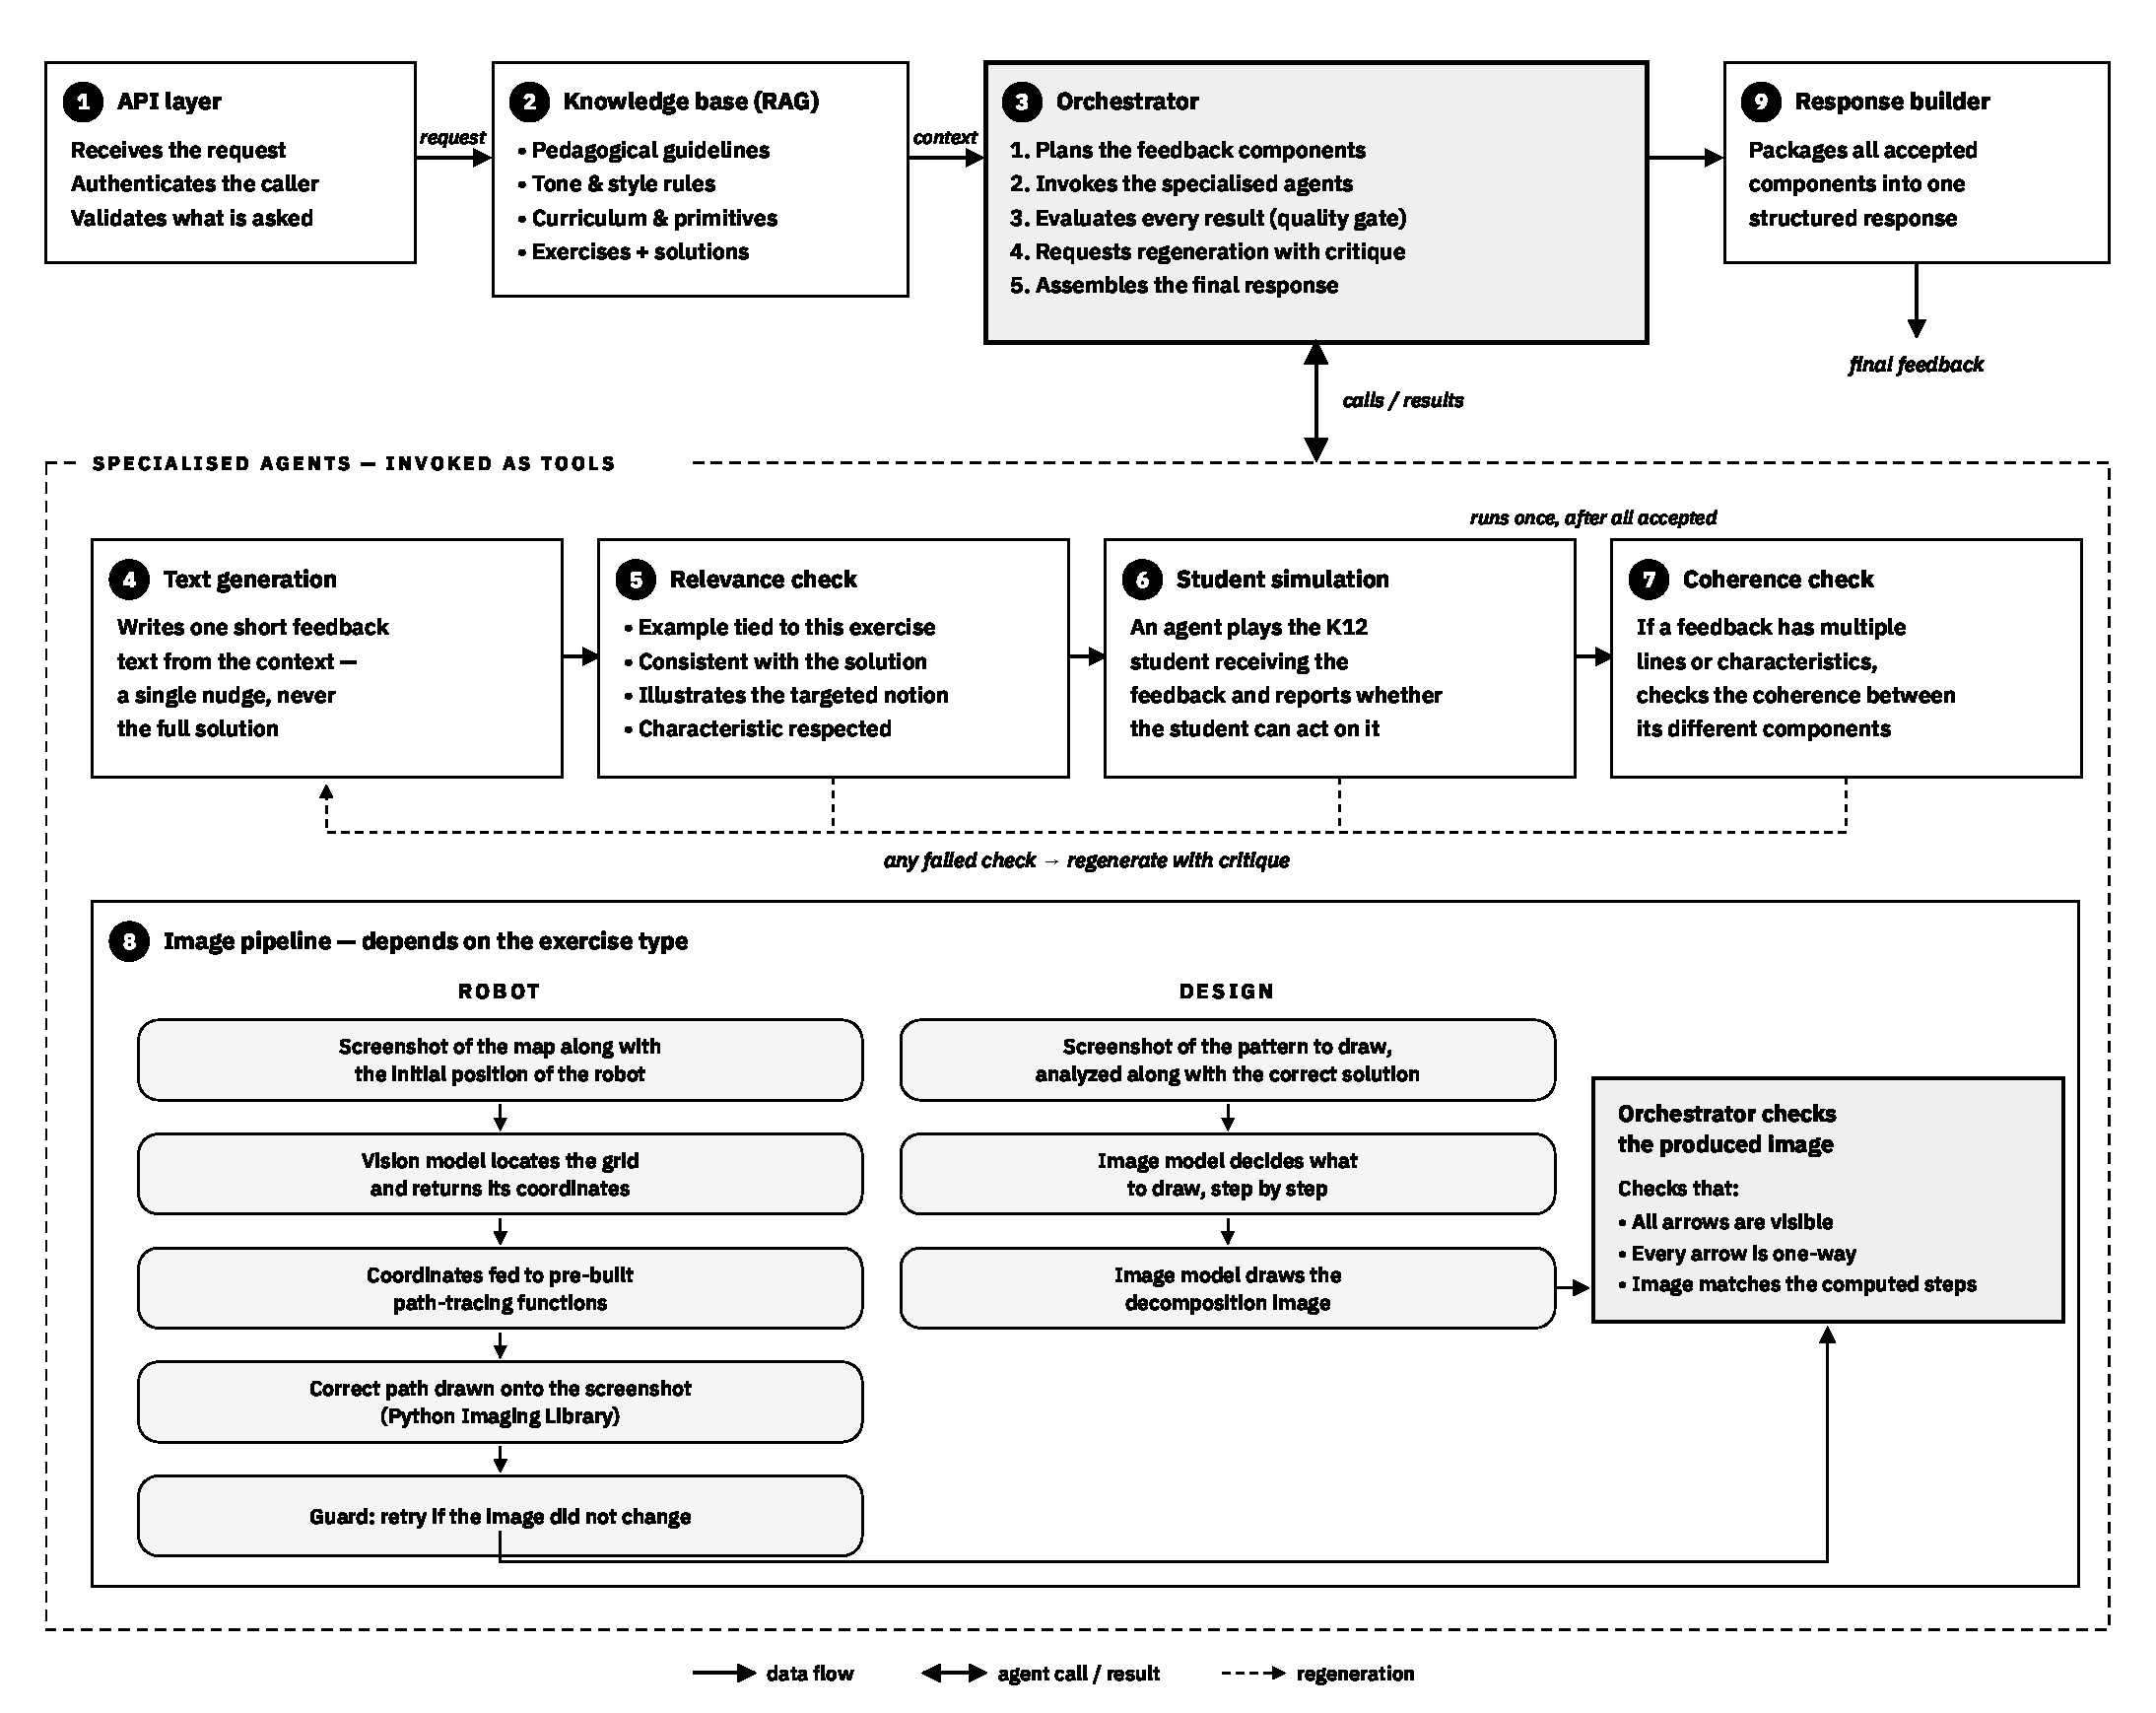
\includegraphics[width=\textwidth]{architecture.pdf}
  \caption{System architecture. A feedback request is authenticated and validated \cmp{1} and grounded with retrieved knowledge \cmp{2}. The orchestrator \cmp{3} invokes the specialised agents \cmp{4}--\cmp{8} as tools and evaluates every result. Each text component follows the workflow \cmp{4}$\rightarrow$\cmp{5}$\rightarrow$\cmp{6}; the coherence check \cmp{7} runs once across all accepted components. Any failed check returns a critique that triggers a targeted regeneration (dashed arrows), within a bounded budget. Visual aids are produced by the exercise-type-specific image pipeline \cmp{8}, and accepted components are packaged into the final response \cmp{9}.}
  \label{fig:architecture}
\end{figure}

\subsection{Agents}
\label{sec:agents}

\textbf{API layer \cmp{1}.} The entry point exposes one endpoint per feedback level. It authenticates administrative callers with JSON Web Tokens and platform integrations with API keys, then validates the request against the constraints of Section~\ref{sec:framework}: a characteristic that requires an error or an exercise context is rejected when that context is absent, before any model is invoked.

\textbf{Knowledge base \cmp{2}.} All generation is grounded in retrieved knowledge rather than in model memory. A vector store, indexed with multilingual sentence embeddings, holds the platform knowledge in chunks: pedagogical guidelines, tone and style rules, the curriculum with its programming primitives, and one chunk per exercise containing its description and reference solutions. At request time, targeted queries retrieve each kind of chunk, and the results are assembled into a single context string given to the orchestrator; when an exercise identifier is supplied, its chunk is parsed back into a structured description and solution set. The reference solutions matter twice: they ground the text generation, and they are the source from which all image geometry is computed.

The choice of a vector store deserves a remark. In our case the platform knowledge carries a strong sequential structure---the curriculum orders notions and exercises along a progression---so the relevant context could, in principle, be fetched by position alone. Other applications of the architecture, however, may have no such ordering; semantic retrieval over a vector store makes the grounding mechanism independent of any structural assumption on the knowledge. Beyond this generality, a vector store is a particularly fitting choice for both modes of use. For dataset curation, it guarantees that every generated feedback is grounded in the same versioned knowledge: thousands of components can be produced in batch against an identical pedagogical context, which keeps the curated corpus homogeneous, and the platform knowledge can be extended---new exercises, revised guidelines---by inserting chunks, without touching prompts, code, or models. For live interaction, retrieval is local and adds negligible latency, and only the chunks relevant to the current request enter the model context, which bounds the cost of each interaction; semantic search also tolerates variation in how an exercise or notion is referred to, across both French and English.

\textbf{Orchestrator \cmp{3}.} A single agent coordinates the whole process through a tool-use loop: it receives the grounded context and the list of components to produce, then alternates between invoking the specialised agents as tools and reasoning over their results. Its system prompt encodes a six-dimension quality gate---length, characteristic purity, register, scope, language, and formatting---with hard violations defined per characteristic. Judgement is calibrated by curated gold examples: every generation result is returned to the orchestrator together with two gold-standard components of the same characteristic, which it must use as calibration anchors for length, purity, register, and scope. When a result fails the gate or any downstream check, the orchestrator writes a targeted critique and re-invokes the generation tool. The orchestrator never writes feedback itself, and the number of regeneration attempts per component is capped independently of its own judgement, so cost and latency stay bounded.

\textbf{Text generation \cmp{4}.} A generation agent writes one short feedback text per component from a characteristic-specific prompt template. The templates embed non-negotiable rules: at most two lines of prose, a single pedagogical nudge that leaves room for discovery, plain text with explicit tags for code references, and never the full solution. Each invocation receives the full grounded context, so the agent always writes with the platform's tone rules and the exercise material at hand.

\textbf{Relevance check \cmp{5}.} When the component carries an example anchored in the exercise, it must pass a two-layer verification. A fast lexical pre-check immediately rejects degenerate examples, such as code that re-defines one of the platform's native primitives---these are always called, never declared. A semantic judge then performs four verifications. First, it extracts the identifiers specific to the exercise (the names of the functions and variables a student would manipulate) and checks that the example actually uses them, rejecting generic snippets that could have been written without knowing the exercise. Second, it checks that the example is consistent with the reference solution and does not contradict it. Third, it checks that the example illustrates the targeted notion, including the form this notion requires: a notion about a student-declared function must be illustrated through that function, whereas a notion about a native primitive must call the primitive directly. Fourth, it checks that the feedback characteristic itself is respected---for an exercise-anchored example, a single introductory sentence that presents the code, followed by the example, without drifting into another characteristic's territory. The verdict is returned as a structured report, with one flag per verification, that the orchestrator can turn into a targeted critique.

\textbf{Student simulation \cmp{6}.} An agent plays the K--12 student receiving the feedback. Given the targeted notion, the exercise, the error if any, and the candidate feedback, it reports whether the student could identify a concrete next step, what that step would be, and what remains unclear; for exercise-anchored examples it also reports whether the example feels connected to the exercise. A negative verdict explains what is missing, which the orchestrator turns into regeneration instructions.

\textbf{Coherence check \cmp{7}.} When a feedback has multiple lines or characteristics, this check---run once, after all components have been individually accepted---verifies the coherence between the different components: no two components may repeat the same point, and together they should cover complementary pedagogical angles. A redundancy failure triggers the regeneration of the less specific component.

\textbf{Image pipeline \cmp{8}.} Visual aids are produced by one of two workflows, selected by exercise type. For \emph{robot} exercises (grid-world navigation), the input is a screenshot of the map along with the initial position of the robot. A vision model locates the grid and returns its coordinates; these coordinates are fed to pre-built path-tracing functions, which compute the correct path from the solution and draw it directly onto the screenshot using the Python Imaging Library. A guard retries the annotation if the resulting image did not change. For \emph{design} exercises (turtle graphics), the input is a screenshot of the pattern to draw, analysed along with the correct solution; an image model decides what to draw, step by step, and then draws the decomposition image. In both workflows the orchestrator checks the produced image before accepting it, verifying that all arrows are visible, that every arrow is one-way, and that the image matches the computed steps. Generative models thus never decide \emph{what} to show---the geometry is computed deterministically from the solution---only how to render it or whether the rendering is faithful.

\textbf{Response builder \cmp{9}.} All accepted components are packaged into one structured response. Each component records the number of generation attempts it required, which serves as a quality signal for monitoring and for curating future gold examples.

\subsection{Model selection}
\label{sec:models}

Each agent role is bound to the model family best supported by current evidence, under one architectural constraint: no model both generates and judges the same artefact, since LLM judges measurably favour their own generations~\cite{panickssery2024llm}. Table~\ref{tab:models} summarises the assignments. Exact model versions are configurable through environment variables; the role assignments, not the versions, are the architectural commitment.

\begin{table}[h]
  \centering
  \small
  \caption{Model assignment per agent role and rationale.}
  \label{tab:models}
  \begin{tabular}{@{}llp{5.6cm}@{}}
    \toprule
    \textbf{Role} & \textbf{Model family} & \textbf{Rationale} \\
    \midrule
    Orchestration \cmp{3}, judging \cmp{5} \cmp{7} & Claude & State-of-the-art agentic tool use~\cite{barres2025tau2,patil2025bfcl}; reliable rubric-based judging~\cite{gu2025judge}. \\
    \addlinespace
    Generation \cmp{4}, simulation \cmp{6} & Mistral & Strong native French for a francophone K--12 audience; low cost per call; disjoint from the judge family~\cite{panickssery2024llm}. \\
    \addlinespace
    Grid localisation \cmp{8} & Claude (vision) & Coordinate grounding in unconstrained interface screenshots. % TODO: cite
    \\
    \addlinespace
    Image generation \cmp{8} & GPT-Image & Instruction-following image generation (exact arrow counts, positions, directions). % TODO: cite
    \\
    \addlinespace
    Retrieval embeddings \cmp{2} & Multilingual MiniLM & Cross-lingual French/English similarity at negligible latency, runs locally~\cite{enevoldsen2025mmteb}. \\
    \bottomrule
  \end{tabular}
\end{table}

\section{Examples}
\label{sec:examples}

\subsection{Robot exercise}
\label{sec:example-robot}

We illustrate the pipeline on a robot exercise. The student must program the robot to reach the goal on a grid map; the request targets the notion of % TODO: KC
, at the exercise level, with the characteristics \charac{logos} and \charac{with\_example\_related\_to\_exercise} (image).
% TODO: finish the robot example — request, generated components, annotated screenshot.

\subsection{Design exercise}
\label{sec:example-design}

We now consider a design exercise. The student must reproduce a turtle-graphics pattern; the request targets the notion of % TODO: KC
, at the exercise level.
% TODO: finish the design example — request, generated components, decomposition image.

\begin{thebibliography}{9}
\bibitem{jolivet} % TODO: add the reference for Sébastien Jolivet's feedback framework.
S.~Jolivet. \emph{(reference to be completed)}.

\bibitem{bk} % TODO: complete this reference (RL-based feedback selection).
\emph{(reference to be completed)}.

\bibitem{panickssery2024llm}
A.~Panickssery, S.~Bowman, and S.~Feng.
LLM evaluators recognize and favor their own generations.
In \emph{Advances in Neural Information Processing Systems (NeurIPS)}, 2024.

\bibitem{barres2025tau2} % TODO: verify authors and venue.
V.~Barres, H.~Dong, S.~Ray, X.~Si, and K.~Narasimhan.
$\tau^2$-Bench: Evaluating conversational agents in a dual-control environment.
\emph{arXiv preprint arXiv:2506.07982}, 2025.

\bibitem{patil2025bfcl} % TODO: verify authors and venue.
S.~G. Patil, H.~Mao, et~al.
The Berkeley Function Calling Leaderboard (BFCL): From tool use to agentic evaluation of large language models.
In \emph{International Conference on Machine Learning (ICML)}, 2025.

\bibitem{gu2025judge} % TODO: verify authors and venue.
J.~Gu, X.~Jiang, Z.~Shi, et~al.
A survey on LLM-as-a-judge.
\emph{arXiv preprint arXiv:2411.15594}, 2025.

\bibitem{enevoldsen2025mmteb} % TODO: verify authors and venue.
K.~Enevoldsen, I.~Chung, I.~Kerboua, et~al.
MMTEB: Massive multilingual text embedding benchmark.
In \emph{International Conference on Learning Representations (ICLR)}, 2025.
\end{thebibliography}

\end{document}
